\chapter{Test Journal: Speed of antenna stand, precision in elevation angle and laser attachment}
\begin{table}[h]
\begin{tabular}{l l}
\textbf{Test participants:} & Mads \& Bang \\
\textbf{Date:}  & 7/12-2016
\end{tabular}
\end{table}

\section*{Purpose}
The purpose of this test is to evaluate the requirements for the mechanical module by measuring the speed of the antenna stand in both azimuth and elevation and comparing the results to the required speed. The precision of the antenna stand's movement in the elevation angle, and whether the antenna stand can support a laser is also tested. \autoref{req:mech_com} is not tested in this setup. 
\section*{Test equipment and components}
The test equipment and components are listed in \autoref{tab_appendix:stand_speed}.
\begin{table}[h]
	\centering
	\caption{List of measurement equipment and components}\label{tab_appendix:stand_speed}
	\begin{tabularx}{\textwidth}{lXXXX}
		Name 					& Brand			& Model 				& AAU-number	\\ \toprule \rowcolor{lightGrey}
		Power supply			& Hameg triple 	& HM7042				& 33902			\\ 
		Antenna stand 	& N/A			& N/A					& N/A \\ \rowcolor{lightGrey}
		Stop watch          	& OnePlus phone & 2                     & N/A \\   
	\end{tabularx}
\end{table}

\section*{Setup}
The test is divided into three parts, using the same setup. The measurement setup is seen on \autoref{fig:motor_speed}.

The first part determines the precision of the antenna stand in the elevation direction. A laser is attached so it is fixed pointing straight ahead compared to the antennas.
The angle that the antenna stand has moved is determined by measuring the distance the laser dot has moved on a wall straight ahead. The distance between the antenna stand and the wall is also measured.

The second part aims to determine the angular speed in the elevation direction by measuring the time it takes for the antennas to move a specific angle. The angle which the antenna stand has moved is derived from the distance the laser dot has moved and the distance from the wall.

The third part aims to determine the speed of the antenna stand in the azimuth direction by measuring the time it takes for it to complete a full revolution at full speed.

\begin{figure} [h]
\centering
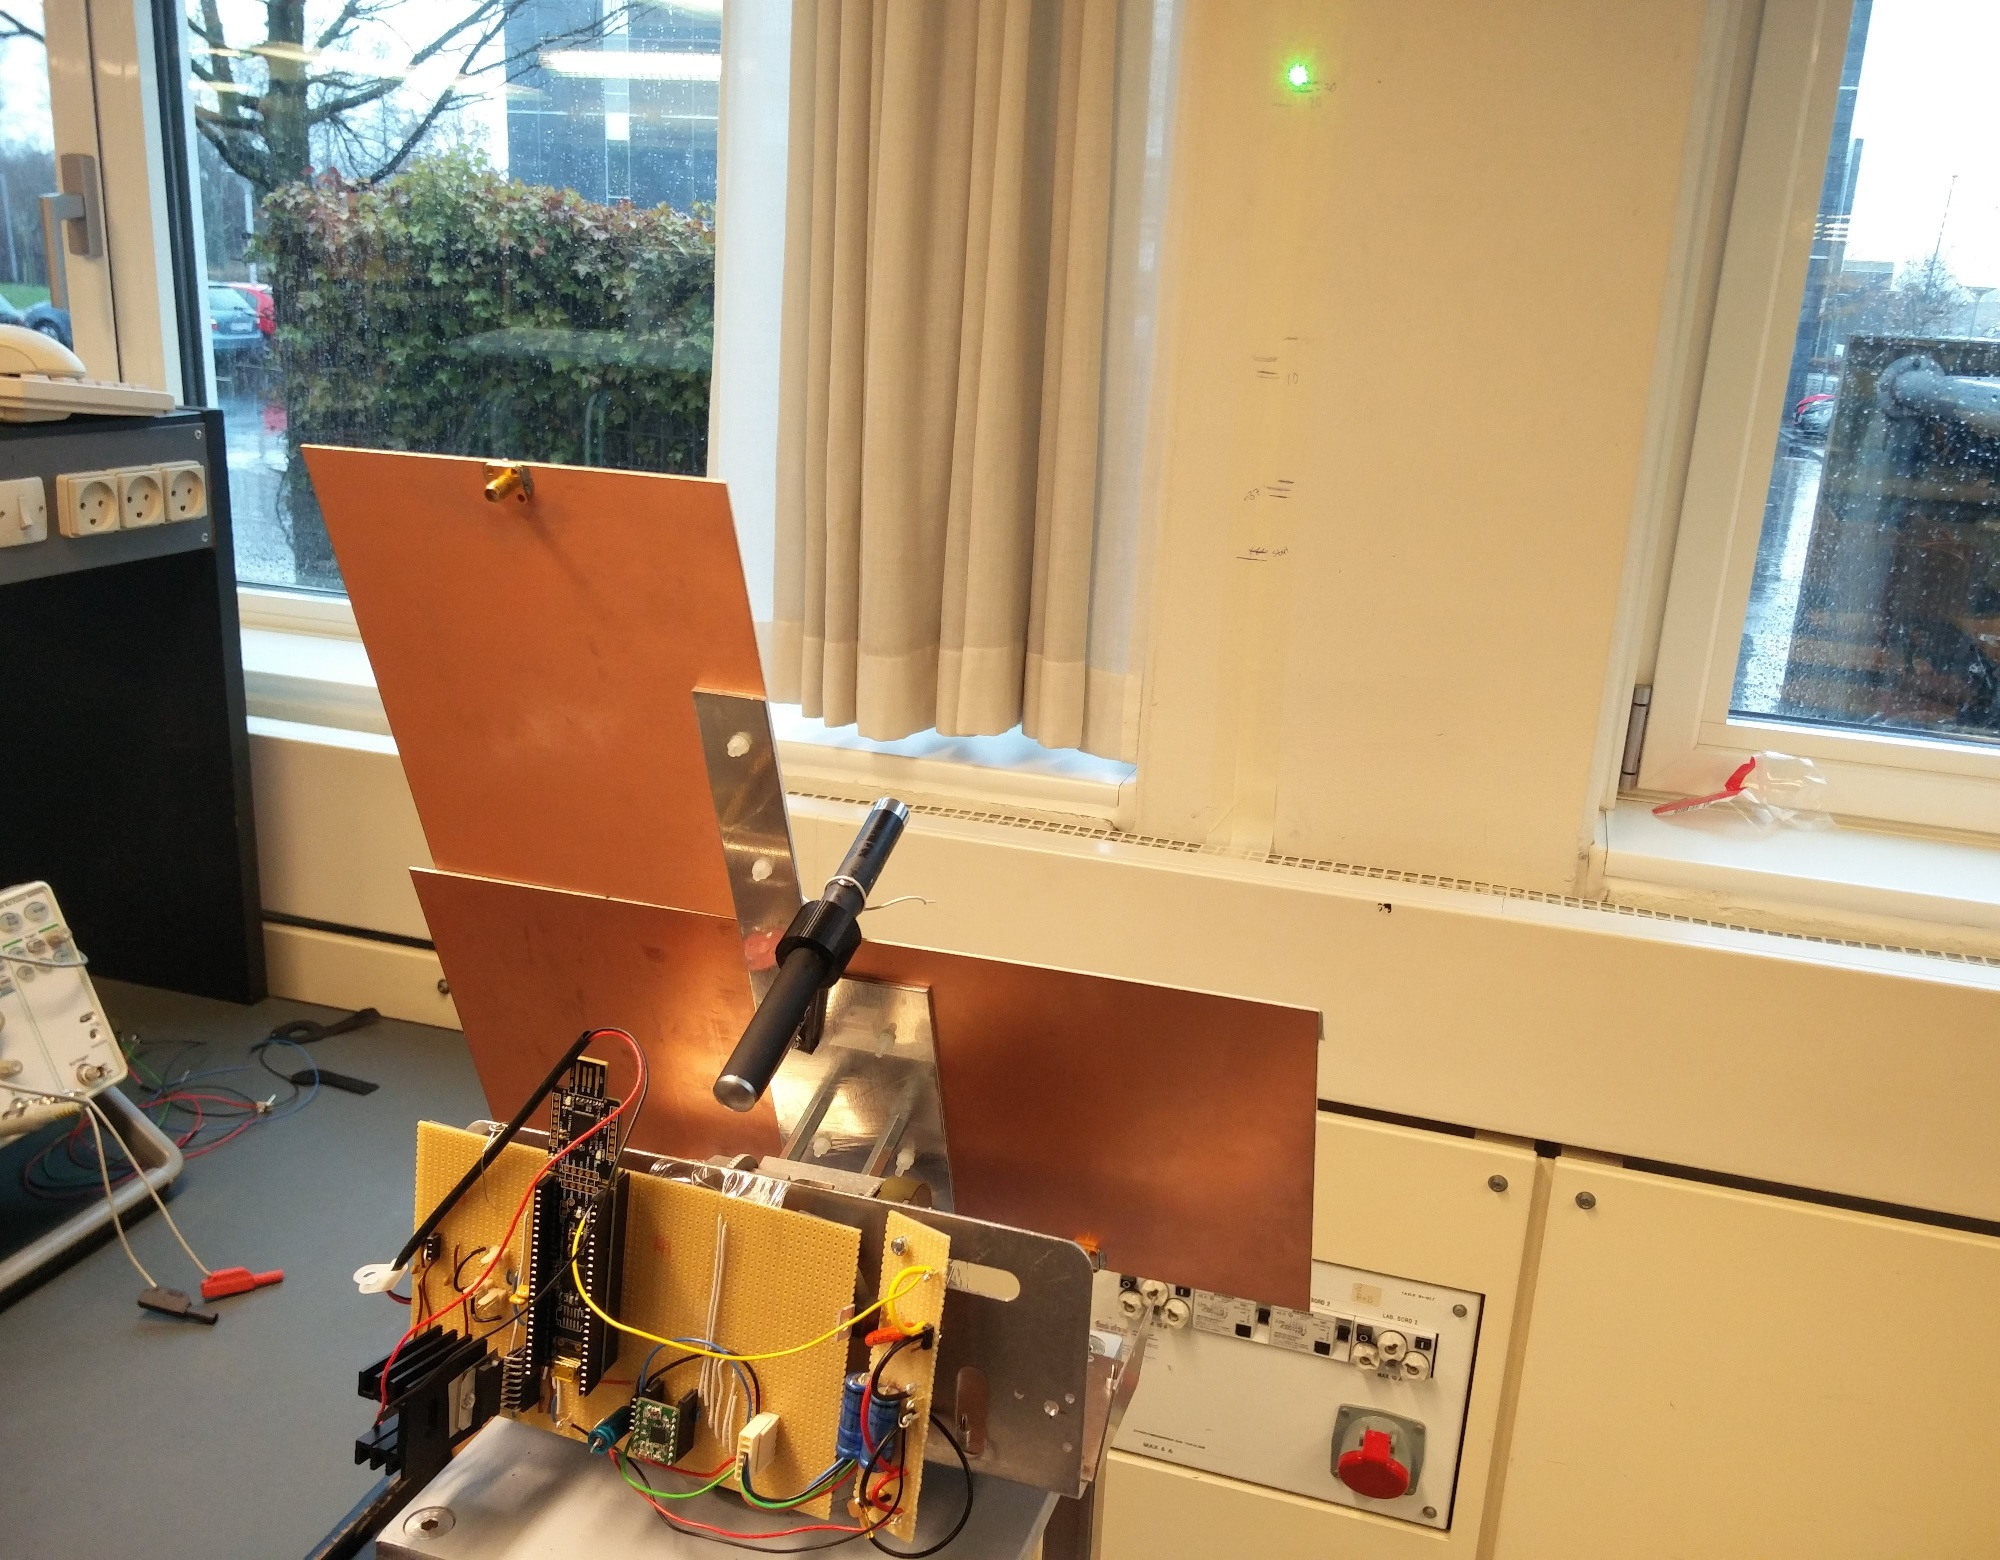
\includegraphics[width=0.6\textwidth]{figures/test/DC_motor_speed}
\caption{Measurement setup.}
\label{fig:motor_speed}
\end{figure}


\section*{Method}
\subsection*{Elevation precision}
A simple sketch of the method can be seen on \autoref{Appendix:fig:Triangle1} where the laser is  rotated around the center point $O$. Initially the laser is pointed directly straight to create a right angled triangle to calculate the precision of the stepper motor. The center of rotation of the stand is placed \SI{1.025}{\meter} from the wall where it is pointing at. The laser is turned on and set to point at the same height as the laser. This is marked as a starting point.

The angle $\theta$ is determined by \autoref{Appendix:speed_eq:test1}.
\begin{equation}\label{Appendix:speed_eq:test1}
\theta = \arctan\left(\frac{h}{L}\right)    
\end{equation}

\begin{figure} [!h]
    \centering
        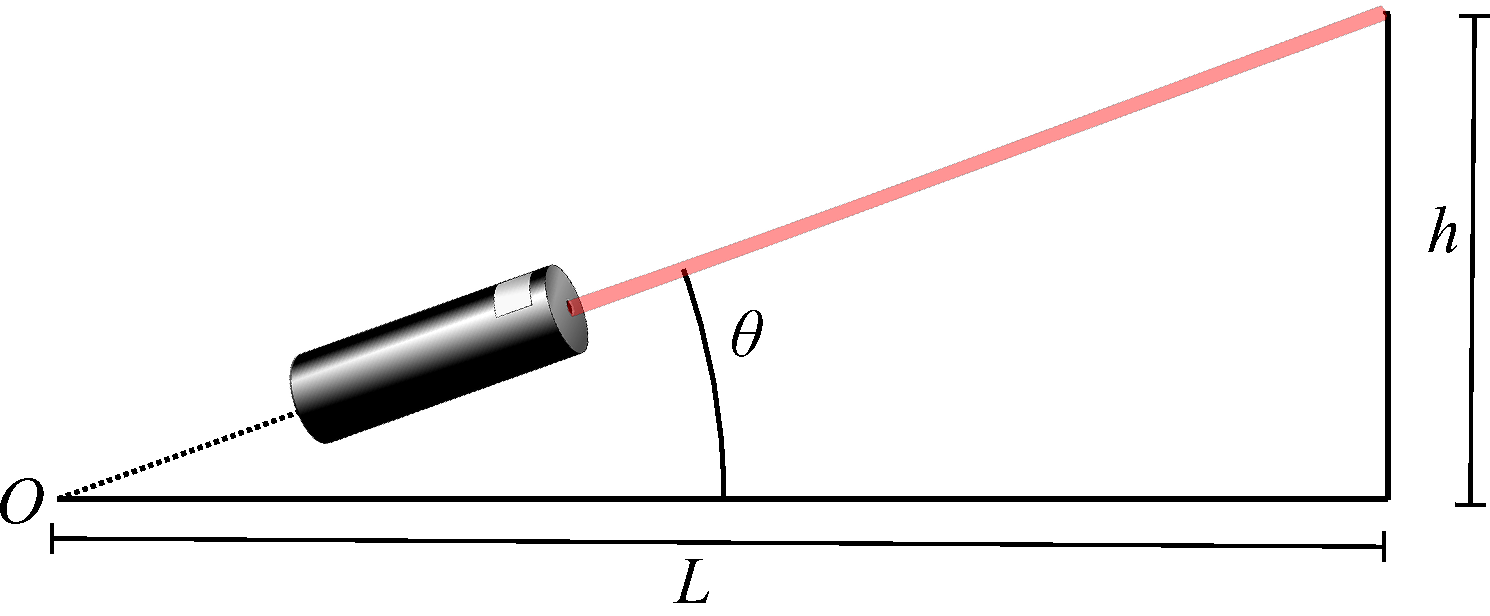
\includegraphics[width=0.6\textwidth]{figures/test/Triangle1}
        \caption{The setup for measuring the positive movement for the elevation angle. The laser rotates around the center point $O$.}
        \label{Appendix:fig:Triangle1}
\end{figure}

To measure the actual angle in the negative direction (downwards) the method is changed to the setup seen on \autoref{Appendix:fig:Triangle2}. Initially the antenna stand is pointed at a defined point and set to move an angle downwards. The distance the laser dot has moved is noted and the angle is derived from \autoref{Appendix:speed_eq:test2}.
\begin{equation}\label{Appendix:speed_eq:test2}
\theta_1 = \arctan\left(\frac{h1}{L}\right)
\theta_2 = \theta - \theta_1 = \arctan\left(\frac{h_1+h_2}{L}\right) - \theta_1
\end{equation}

\begin{figure} [h]
    \centering
        \includegraphics[width=0.6\textwidth]{figures/test/Triangle2}
        \caption{The setup for measuring the negative movement for the elevation angle. The laser rotates around the center point $O$.}
        \label{Appendix:fig:Triangle2}
\end{figure}

It is not possible to go above \SI{37}{\degree} because of limitations in the implementation of the stepper motor controller on the \gls{psoc}.
\begin{enumerate}
\item Set the controller to move a specific angle.
\item Let the stand settle after the rotation.
\item Measure the distance the laser is pointing to the start mark.
\item Note the distance.
\item Do step 1 to 4 with \SI{0}{\degree}, \SI{10}{\degree}, \SI{20}{\degree}, \SI{30}{\degree} and \SI{37}{\degree} in both direction.
\end{enumerate}


\subsection*{Speed in elevation angle}
The speed of the elevation angle is determined by having the stepper motor move to a known angle which is already determined from previous tests. The time it takes for the stand to move to the angle is timed using a stopwatch.
\begin{enumerate}
\item Set the controller to move \SI{39}{\degree}.
\item Take time for the stepper motor to rotate.
\item Take 10 measurements.
\item Note the time.
\end{enumerate}

\subsection*{Speed in azimuth direction}
The speed of the azimuth angle is determined by having the DC motor run full speed using the designed DC motor controller and the driver. The speed is measured by timing how long it takes to complete a round.
\begin{enumerate}
\item Start the rotation of the stand in the azimuth direction and let it settle.
\item Measure the time it takes to rotate a round.
\item Take 10 measurements.
\item Note the time.
\end{enumerate}

\subsection*{Laser support}
The antenna stand is set to move at full speeds while the laser is attached.
\begin{enumerate}
\item Set the controller to move \SI{360}{\degree} clockwise and counter clockwise at maximum speed.
\item Redo step 1 three times.
\item Set the controller to move \SI{90}{\degree} up and down full steps.
\item Redo step 3 three times.
\item Check if the laser is in same position
\end{enumerate}

\clearpage

\section*{Raw data}
The data from the tests is given in Tables \ref{tab_appendix:elevation_test_a}, \ref{tab_appendix:elevation_test_b}, \ref{tab_appendix:speed_azimuth} and \ref{tab_appendix:speed_elevation}.
\begin{table}[h!]
	\centering
	\caption{Measurements of the precision in the positive elevation angle.} \label{tab_appendix:elevation_test_a}
	\begin{tabularx}{\textwidth}{lXXX}
		Input angle [\si{\degree}]     & Height [\si{\meter}] &  Measured angle \si{\degree} & Deviation [\%]  \\ \toprule  \rowcolor{lightGrey} 
		0  &  0    & 0     & 0  \\
		10 & 0.165 & 9.145 & -8.55	\\\rowcolor{lightGrey}
		20 & 0.366 & 19.650 & -1.75 \\ 
		30 & 0.60 & 30.343 & 1.14\\ \rowcolor{lightGrey}
		37 & 0.84 & 39.335 & 6.31 \\ 
	\end{tabularx}
\end{table}

\begin{table}[h!]
	\centering
	\caption{Measurements of the precision in the negative elevation angle.} \label{tab_appendix:elevation_test_b}
	\begin{tabularx}{\textwidth}{lXXXXX}
		Input angle [\si{\degree}]    & Start height [\si{\meter}] &  Height diffrence (h1) [\si{\meter}] & Height (h2)[\si{\meter}] & Measured angle [\si{\degree}] & Deviation [\%] \\ \toprule  \rowcolor{lightGrey} 
		-10 & 0.996 & 0.655 & 0.341 & 11.598	& 15.98\\
		-20 & 0.996 & 0.396 & 0.6   & 23.054 & 15.27\\ \rowcolor{lightGrey}
		-30 & 0.996 & 0.197 & 0.799 & 33.299 & 11.00\\ 
		-37 & 0.996 & 0.072 & 0.924 & 40.160 & 8.54\\ 
	\end{tabularx}
\end{table}
 
\begin{table}[h!]
	\centering
	\caption{Results of the speed measurements in the azimuth direction.}

	\begin{tabularx}{\textwidth}{lXX}\label{tab_appendix:speed_azimuth}
		Test 				& Speed in azimuth direction [\si{\second\per round}]			&  Speed in azimuth direction [\si{\radian\per\second]}			\\ \toprule \rowcolor{lightGrey}
		1	& 2.32 & 2.71						\\
		2	& 2.37	& 2.65		\\ \rowcolor{lightGrey}
		3	& 2.38 & 2.64 \\
		4	& 2.26 & 2.78 \\ \rowcolor{lightGrey}
		5 	& 2.42 & 2.60 \\
		6	& 2.37 & 2.65 \\\rowcolor{lightGrey}
		7	& 2.43 & 2.59 \\
		8	& 2.32 & 2.71 \\ \rowcolor{lightGrey}
		9	& 2.37 & 2.65 \\
		10	& 2.33 & 2.70 \\\rowcolor{lightGrey}
		\textbf{Average} & \textbf{2.357} & \textbf{2.67} 
	\end{tabularx}
\end{table}

\begin{table}[h!]
	\centering
	\caption{Results of the speed measurements in the elevation direction.}\label{tab_appendix:speed_elevation}

	\begin{tabularx}{\textwidth}{lXX}
		Test 				& Speed in elevation direction [\si{\second\per 39.3 \degree}]		&  Speed in elevation direction [\si{\radian\per\second]}			\\ \toprule \rowcolor{lightGrey}
		1	& 1.52 & 0.451						\\
		2	& 1.26 & 0.544		\\ \rowcolor{lightGrey}
		3	& 1.47 & 0.467 \\
		4	& 1.41 & 0.486 \\ \rowcolor{lightGrey}
		5 	& 1.28 & 0.536 \\
		6	& 1.31 & 0.524 \\\rowcolor{lightGrey}
		7	& 1.34 & 0.512 \\
		8	& 1.24 & 0.553 \\ \rowcolor{lightGrey}
		9	& 1.24 & 0.553 \\
		10	& 1.25 & 0.549 \\\rowcolor{lightGrey}
		\textbf{Average} & \textbf{1.332} & \textbf{0.518} 
	\end{tabularx}
\end{table}

\section*{Data processing}
The precision  of the angle is calculated in \autoref{tab_appendix:elevation_test_a} and  \autoref{tab_appendix:elevation_test_b}. The angle deviates a lot from the input angle and is more precise in the positive direction. Moving in the positive elevation angle requires the stepper motor to carry a lot of weight and is similarly dragged down in the negative elevation angle.
The best precision is achieved at \SI{30}{\degree} movement in the positive elevation angle which is \SI{0.34}{\degree} which is \SI{5.99}{\milli\radian}.

The stand is not able to point in the elevation angle with a precision of less than \SI{2}{\milli\radian} without a feedback loop. Despite this lack of precision, the entire system might compensate for this using the feedback loop with the tracking system since the elevation angle can still be controlled in smaller steps than \SI{2}{\milli\radian} as the precision stated in \autoref{req:mech_precision}.


\section*{Conclusion}
\subsection*{Angle precision}
The stepper motor rotate a given angle with a deviation up to 16\%. The feedback control system will correct the deviation. The elevation angle cannot be as precisely controlled without feedback as specified in \autoref{req:mech_precision}.
But is still able to move in smaller steps than \SI{2}{\milli\radian} so using the feedback from the tracking module, the precision might still be achievable. Without feedback from the tracking module it is not possible to test the angle precision for the azimuth angle. 

\subsection*{Speed}
The speed of the azimuth angle is \SI{2.67}{\radian\per\second} which is more then the required speed. The speed of the elevation angle is \SI{0.518}{\radian\per\second} which is less then the required speed. Several solution could speed up the movement in the elevation direction. Another stepper motor, higher voltage or a lighter antenna stand might allow for a higher stepping frequency and therefore higher speed.

\subsection*{Laser support}
The laser attachment is stable.

